\documentclass[letterpaper, 12pt]{article}
\usepackage[letterpaper, top=2.5cm, bottom=2.5cm, left=3cm, right=3cm]{geometry} %margenes
\usepackage[utf8]{inputenc} %manejo de caracteres especiales
\usepackage[spanish]{babel} %manejo de encabezados de inglés a español
\usepackage{fancyhdr} %formato de los encabezados de página
\usepackage{ragged2e} %alineado real justficado
\usepackage{graphicx} %manejo de imagenes
\usepackage{amsmath} %manejo de notación matemática
\usepackage{mathtools} %manejo de notación matemática
\usepackage{blindtext} %texto de relleno
\usepackage{cancel} %permite la simbolización de cancelación de terminos
\usepackage{enumitem}[shortlabels] %listas con letras
\usepackage{amssymb} %manejo de simbolog►1a matematica
\usepackage{mhchem}
\usepackage[backend=biber]{biblatex}\addbibresource{referencias.bib}

\pagestyle{fancy}
\fancyhf{}
\rfoot{\thepage}

\nocite{*}

\begin{document}
\begin{titlepage}
    \begin{figure}[ht]
        \centering
        
\includegraphics[width=15cm]{logosITT.png}
    \end{figure}
    \centering
    {\scshape\LARGE Tecnológico Nacional de México\\Instituto Tecnológico de Tijuana\par}
    \vspace{1cm}
    {\scshape\Large Química\par}
    \vspace{1cm}
    {\scshape\Large Unidad 1\par}
    \vspace{1.5cm}
    {\huge\bfseries Rayos anódicos\par}
    \vspace{2cm}
    {\Large\itshape C. Abraham Jhared Flores Azcona\\19211640\par}
    \vfill
    Profesor: \par
    Dr. Luis Ernesto Solís Delgado
    
    \vfill

    {\large 12 de octubre del 2020}
\end{titlepage}

        \begin{justify}
    \thispagestyle{empty}
    \section*{Rayos anódicos}
    \subsection*{¿Qué son?}
    Conocidos tambien como \emph{rayos canales o positivos}. Son haces de rayos constituidos por cationes atómicos o moleculares (ionies con carga positiva)
    que se dirigen hacia el electrodo negativo en un \emph{tubo de Crookes}. Dichos rayos se originan cuando los electrones que van desde el cátodo hacia el ánodo, chocan con los átomos del gas encerrado en el tubo de Crookes.
    Como las particulas del mismo signo se repelen, los eletrones que van hacia el anodo arrancan a su paso los electrones presentes en la corteza de los átomos de gas. Así, los átomos que se han quedado cargados de manera positiva
    son atraídos hacia el cátodo.
    \begin{center}
        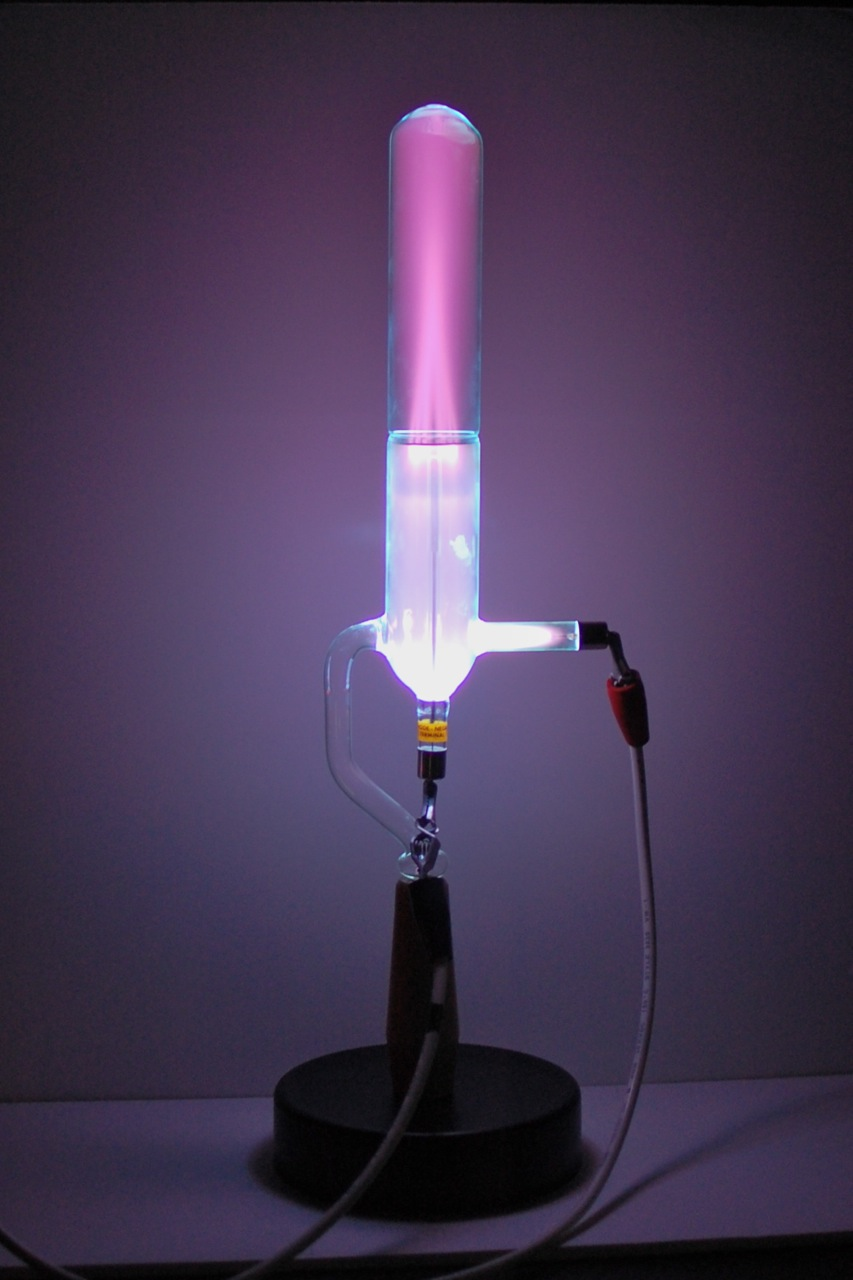
\includegraphics[width=6cm]{tube.jpg}
    \end{center}
    \subsection*{Propiedades}
    \begin{itemize}
        \item Viajan en linea recta.
        \item Consisten de partículas materiales.
        \item Son desviados en campos electricos y magneticos.
        \item La naturaleza o la \emph{razón \(e/m\)} de estos rayos depende de la naturaleza del gas presente en el tubo para rayos catódicos.
        \item Sus partículas simplemente son iones gaseososo positivamente cargados.
        \item Las partículas positivamente cargadas \emph{contienen una carga igual al multiplo de la unidad fundamental de carga electrica: }\(n\times 10^{-19}C,\,\text{Ej: }\,\ce{Ca^2+}=2\times 10^{-19}C\).
    \end{itemize}
        \end{justify}

        \newpage
        \thispagestyle{empty}
        \addcontentsline{toc}{section}{Referencias}
        \printbibliography
\end{document}